\documentclass[12pt,a4paper]{article}

\usepackage{fontspec}
\usepackage{geometry}
\usepackage{hyperref}
\usepackage{booktabs}
\usepackage{longtable}
\usepackage{xcolor}
\usepackage{listings}
\usepackage{graphicx}
\usepackage{microtype}
\usepackage{array}
\usepackage[font=small,labelfont=bf]{caption}

\geometry{margin=2.4cm}
\setmainfont{Latin Modern Roman}
\setsansfont{Latin Modern Sans}
\setmonofont{Latin Modern Mono}
\hypersetup{colorlinks=true, linkcolor=black, urlcolor=blue}
\setlength{\parskip}{0.45em}
\setlength{\parindent}{0pt}
\setlength{\emergencystretch}{2em}

\definecolor{esiBlue}{HTML}{123F68}
\definecolor{esiAccent}{HTML}{1976A3}
\definecolor{esiText}{HTML}{2B2F36}

\lstset{
  basicstyle=\ttfamily\small,
  breaklines=true,
  frame=single,
  columns=fullflexible,
  backgroundcolor=\color{gray!8}
}

\begin{document}

\pagenumbering{gobble}
\begin{titlepage}
  \centering
  \vspace*{0.4cm}
  
\includegraphics[width=0.32\linewidth]{screenshots/esi_logo.png}\par
  \vspace{0.7cm}
  {\Large ESI -- \'{E}cole nationale Sup\'erieure d'Informatique\par}
  \vspace{0.2cm}
  {\color{esiText}SIQ -- Base de donn\'ees avanc\'ees\par}
  \vspace{1.2cm}
  {\color{esiBlue}\rule{\linewidth}{1.2pt}\par}
  \vspace{0.7cm}
  {\Huge\bfseries\color{esiBlue}Moteur de recherche s\'emantique et analytique sur des logs massifs Big Data\par}
  \vspace{0.5cm}
  {\Large Rapport technique\par}
  \vspace{0.7cm}
  {\color{esiAccent}\rule{0.64\linewidth}{0.8pt}\par}
  \vfill
  \begin{minipage}{0.92\linewidth}
  \renewcommand{\arraystretch}{1.35}
  \begin{tabular}{@{}>{\bfseries}p{0.22\linewidth}p{0.72\linewidth}@{}}
    Auteurs & Tati Youcef -- \texttt{my\_tati@esi.dz}\\
            & Mostefai Mounir Sofiane -- \texttt{mm\_mostefai@esi.dz}\\
    Encadrement & Ens. Amrouche Karima -- \texttt{k\_amrouche@esi.dz}\\
  \end{tabular}
  \end{minipage}
  \vfill
  {\large Ann\'ee universitaire 2025--2026\par}
\end{titlepage}

\pagenumbering{roman}
\tableofcontents
\newpage
\pagenumbering{arabic}

\begin{abstract}
Ce rapport présente la conception et la réalisation d'une plateforme Big Data de recherche
sémantique appliquée aux logs OpenSSH de LogHub-2.0. La solution combine Apache Spark pour le
prétraitement batch, PostgreSQL avec pgvector pour le stockage vectoriel indexé,
Sentence-Transformers pour la représentation sémantique, FastAPI pour l'exposition des services et
Streamlit pour la visualisation interactive. Le système traite 638 947 entrées, fournit une
recherche sémantique, une recherche lexicale de référence, l'identification de groupes d'erreurs
récurrentes, l'analyse temporelle et une évaluation comparative de plusieurs modèles
d'embeddings.
\end{abstract}

\textbf{Mots-clés :} Big Data, logs, recherche semantique, pgvector, Apache Spark,
Sentence-Transformers, analyse d'erreurs.

\section{Introduction}

Les infrastructures modernes produisent des volumes importants de journaux d'execution. Dans un
systeme distribue, ces journaux proviennent de machines, services, processus et utilisateurs
differents. Leur exploitation par recherche textuelle simple reste limitee : une meme panne peut
etre formulee par plusieurs messages proches, et une requete par mot-cle peut ignorer des logs
pertinents lorsque les termes exacts ne sont pas presents.

Cette etude presente une plateforme Big Data capable d'ingerer un grand volume de logs, de les
structurer avec Apache Spark, de transformer les messages en vecteurs semantiques, de stocker ces
vecteurs dans PostgreSQL avec pgvector, puis de fournir des fonctions de recherche et d'analyse.
L'analyse porte sur une chaine complete, reproductible et observable, depuis le traitement batch
jusqu'aux resultats consultables par API et interface web.

La solution s'appuie exclusivement sur des composants open source : Python, Apache Spark,
PostgreSQL, pgvector, Sentence-Transformers, FastAPI et Streamlit. Le rapport decrit le jeu de
donnees, les choix de conception, le schema de stockage, les fonctions de recherche et les resultats
observes.

\section{Jeu de donnees}

Le dataset utilise est OpenSSH de LogHub-2.0. Il contient 638 947 entrees brutes dans l'extraction
locale, ce qui fournit un volume suffisant pour evaluer un pipeline de recherche sur logs massifs.
Le depot local contient trois fichiers principaux :

\begin{longtable}{p{0.42\linewidth}p{0.46\linewidth}}
\toprule
Fichier & Role\\
\midrule
\texttt{OpenSSH\_full.log} & Logs bruts au format syslog, avec mois, jour, heure, hote, service et message.\\
\texttt{OpenSSH\_full.log\_structured.csv} & Version structuree fournie par LogHub : identifiant de ligne, contenu, identifiant d'evenement et template.\\
\texttt{OpenSSH\_full.log\_templates.csv} & Liste des templates d'evenements et leurs occurrences.\\
\bottomrule
\end{longtable}

Un exemple de ligne brute est :

\begin{lstlisting}
Dec 10 06:55:48 LabSZ sshd[24200]: Failed password for invalid user webmaster from 173.234.31.186 port 38926 ssh2
\end{lstlisting}

La version structuree separe le contenu metier du prefixe syslog. Elle fournit aussi un
\texttt{EventId} et un \texttt{EventTemplate}. Ces templates sont importants car ils reduisent le
bruit des valeurs variables comme adresses IP, ports, noms d'utilisateurs et identifiants de
processus.

\section{Architecture generale}

L'architecture suit une chaine batch classique adaptee a un contexte Big Data :

\begin{lstlisting}
Logs OpenSSH
  -> Pretraitement Spark
  -> CSV/Parquet traites
  -> PostgreSQL + pgvector
  -> API FastAPI
  -> Interface Streamlit
\end{lstlisting}

Spark est utilise pour charger les fichiers volumineux, parser les prefixes syslog, joindre le log
brut avec le CSV structure, normaliser les messages et produire des sorties persistantes. PostgreSQL
stocke les logs nettoyes et une table vectorielle des messages normalises distincts. pgvector ajoute
le type \texttt{vector(384)} et l'index HNSW pour la recherche approximative de voisins proches.
FastAPI expose les fonctionnalites sous forme d'API HTTP, et Streamlit fournit la visualisation
interactive.

La separation entre pipeline, base, API et interface rend la solution reproductible : le pipeline peut
etre lance en ligne de commande, l'API peut etre testee seule, et l'interface consomme uniquement les
endpoints publics.

\section{Pretraitement Big Data}

La commande \texttt{tp5-log-search prepare-data} execute le pretraitement Spark. Le traitement lit le
fichier brut, associe un numero de ligne, puis joint ce flux avec le CSV structure par
\texttt{LineId}. Cette strategie permet de conserver les informations temporelles du log brut et les
templates fournis par LogHub.

Les champs extraits sont :

\begin{itemize}
  \item \texttt{line\_id}, identifiant stable de la ligne ;
  \item \texttt{log\_timestamp}, timestamp reconstruit avec une annee configurable ;
  \item \texttt{host}, \texttt{service}, \texttt{process\_id} ;
  \item \texttt{level}, niveau heuristique : INFO, WARNING, ERROR ou CRITICAL ;
  \item \texttt{raw\_message}, message original ;
  \item \texttt{normalized\_message}, message normalise vectorise ;
  \item \texttt{event\_id} et \texttt{event\_template}.
\end{itemize}

Le fichier OpenSSH ne contient pas l'annee. Pour permettre les analyses temporelles, le pipeline
utilise une variable \texttt{LOG\_YEAR}, fixee par defaut a 2024. Cette hypothese est explicite,
configurable et ne modifie pas l'ordre relatif des evenements.

Le resultat est ecrit sous deux formats. Le CSV sert au chargement rapide dans PostgreSQL avec
\texttt{COPY}. Le Parquet conserve une sortie analytique compacte et partitionnee par niveau de log,
utile pour des analyses Spark supplementaires.

\section{Schema de stockage}

Le schema relationnel est centre sur trois tables :

\begin{longtable}{p{0.25\linewidth}p{0.65\linewidth}}
\toprule
Table & Description\\
\midrule
\texttt{event\_templates} & Dictionnaire des templates LogHub et nombre d'occurrences annonce.\\
\texttt{log\_entries} & Lignes de logs nettoyees, metadonnees temporelles, niveau et message.\\
\texttt{message\_embeddings} & Messages normalises distincts, occurrences et vecteurs semantiques indexes.\\
\texttt{pipeline\_runs} & Trace d'execution du pipeline complet.\\
\bottomrule
\end{longtable}

La colonne vectorielle principale est stockee dans \texttt{message\_embeddings} :

\begin{lstlisting}
embedding VECTOR(384)
\end{lstlisting}

La dimension 384 correspond au modele \texttt{sentence-transformers/all-MiniLM-L6-v2}. Les index
relationnels couvrent le niveau, le temps, l'evenement et la recherche textuelle par trigrammes. La
recherche semantique repose sur :

\begin{lstlisting}
CREATE INDEX message_embeddings_embedding_hnsw_idx
ON message_embeddings USING hnsw (embedding vector_cosine_ops);
\end{lstlisting}

L'index HNSW est adapte a la recherche de similarite a grande echelle car il evite un parcours
sequentiel complet pour chaque requete. La distance utilisee est le cosinus, coherente avec les
embeddings normalises.

\section{Details d'implementation}

Le code source est organise comme un package Python installable. Cette organisation evite les
scripts isoles difficiles a maintenir et donne une base logicielle claire et modulaire. Les
modules principaux sont separes par responsabilite : configuration, pretraitement Spark, acces base
de donnees, embeddings, recherche, analytique, API, interface et CLI.

Le module de configuration lit les variables d'environnement depuis \texttt{.env}. Les chemins sont
resolus relativement a la racine du depot afin que les commandes fonctionnent depuis n'importe quel
repertoire. Les valeurs par defaut pointent vers le dataset OpenSSH deja extrait dans
\texttt{data/raw/OpenSSH}.

Le module Spark evite de supposer que le CSV structure contient toutes les informations utiles. Il
reconstruit les metadonnees systeme depuis le log brut, puis joint ces informations avec les
templates LogHub. Cette decision conserve a la fois la richesse temporelle du fichier brut et la
qualite du parsing fourni par LogHub.

Le chargement PostgreSQL utilise \texttt{COPY} plutot que des insertions ligne par ligne. Pour un
dataset de plusieurs centaines de milliers de lignes, cette difference est importante : \texttt{COPY}
reduit le temps de chargement et limite la charge cote client Python. Les commandes peuvent etre
relancees car le pipeline initialise le schema puis recharge les tables applicatives de maniere
deterministe.

La recherche semantique est encapsulee dans un module dedie. L'API et l'interface n'ont donc pas a
connaitre les details SQL de pgvector. Cette separation facilite les tests et permettrait de changer
le modele d'embedding ou la base vectorielle sans reecrire l'interface.

\section{Choix de conception}

Plusieurs choix ont ete faits pour concilier performance locale, reproductibilite et clarte
operationnelle. Le premier choix est d'utiliser PostgreSQL comme base unique pour les donnees
relationnelles et vectorielles. Cette approche simplifie l'exploitation : les filtres temporels,
niveaux de severite, templates et vecteurs sont interroges dans le meme systeme.

Le deuxieme choix est de vectoriser les messages normalises plutot que chaque message brut
independamment. Sur un dataset de logs structures, les templates representent le sens operationnel
des evenements, tandis que les valeurs variables representent souvent des parametres. Cette
vectorisation rend les groupes d'erreurs plus stables et accelere fortement l'indexation.

Le troisieme choix est de conserver une recherche par mots-cles. Elle ne remplace pas la recherche
semantique, mais elle reste pertinente pour des investigations precises. Par exemple, une adresse IP
ou un port doit etre retrouve lexicalement. La comparaison entre les deux methodes montre donc leur
complementarite.

Le dernier choix est de fournir une API en plus de l'interface. Cette separation explicite le
contrat applicatif et evite de coupler l'interface utilisateur aux details SQL. Avec FastAPI, la
interface web, les tests et d'eventuels clients externes consomment le meme contrat.

\section{Vectorisation}

La vectorisation est realisee avec Sentence-Transformers. La commande
\texttt{tp5-log-search embed} charge le modele, recupere les messages normalises distincts non encore
vectorises, calcule les embeddings par lots, puis les insere dans la table \texttt{message\_embeddings}.

Cette approche est volontaire : la table vectorielle ne contient pas un vecteur par ligne brute,
mais un vecteur par message normalise distinct, generalement issu du template LogHub. Les lignes
brutes restent toutes conservees dans \texttt{log\_entries} et gardent leurs timestamps, niveaux,
identifiants, hote et message original. La liaison entre une ligne et son vecteur se fait par
\texttt{normalized\_message}.

Ce choix est adapte aux logs structures. Dans OpenSSH, beaucoup de lignes partagent le meme template
et ne different que par des valeurs variables comme l'adresse IP, le port ou le nom d'utilisateur.
Calculer et stocker un embedding duplique pour chaque ligne brute gaspillerait du temps CPU et de
l'espace disque sans ajouter beaucoup de signal semantique. En vectorisant les templates
normalises, les 638 947 logs restent recherchables par jointure avec une table vectorielle compacte
et indexee, tout en conservant la possibilite d'afficher chaque occurrence originale.

Les vecteurs sont normalises cote modele. La similarite retournee par l'API est :

\begin{lstlisting}
1 - (embedding <=> query_embedding)
\end{lstlisting}

ou \texttt{<=>} est l'operateur de distance cosinus de pgvector.

\section{Recherche et analyse}

La plateforme expose quatre familles de fonctionnalites.

\subsection{Recherche semantique}

L'utilisateur formule une requete en langage naturel, par exemple :

\begin{lstlisting}
brute force ssh authentication failure
\end{lstlisting}

Le systeme vectorise cette requete, interroge pgvector et retourne les logs les plus proches. Cette
recherche peut retrouver des messages pertinents meme si les mots exacts ne sont pas presents.

\subsection{Recherche par mots-cles}

La recherche par mots-cles utilise \texttt{ILIKE} et l'index trigramme. Elle sert de baseline pour
comparer les resultats avec la recherche semantique. Cette comparaison met en evidence les limites
d'une recherche lexicale stricte sur des logs variables.

\subsection{Logs similaires}

L'endpoint \texttt{/logs/\{id\}/similar} recupere le vecteur d'un log deja indexe, puis cherche ses
voisins les plus proches. Cette fonction facilite l'investigation d'incidents en retrouvant les logs
similaires a une erreur critique donnee.

\subsection{Analytique}

Les groupes d'erreurs frequentes sont calcules par agregation sur \texttt{event\_id},
\texttt{event\_template} et \texttt{level}. L'evolution temporelle agr\`ege les logs par heure ou par
jour. Lorsqu'une requete semantique est fournie, le systeme identifie d'abord les evenements les plus
proches, puis calcule leur evolution sur l'ensemble de la base.

\section{Interface de visualisation}

L'interface Streamlit est organisee en cinq onglets : recherche, comparaison, logs similaires,
analytique et benchmarks. Elle consomme l'API FastAPI et n'accede jamais directement a la base.
Cette separation est importante pour garder une architecture claire et testable.

La page d'accueil affiche les indicateurs principaux : nombre total de logs, couverture de
vectorisation, nombre d'evenements et periode observee. Les tableaux de resultats affichent les
identifiants de logs, timestamps, niveaux, evenements, similarites et messages bruts. Les analyses
recurrences et temporelles utilisent des graphiques Plotly. L'onglet benchmarks complete
l'observation du systeme avec les tailles disque, la latence des requetes, un score de coherence
top-k et une comparaison de plusieurs modeles Sentence-Transformers.

\section{Reproductibilite}

La plateforme est pilotee par une CLI unique :

\begin{lstlisting}
tp5-log-search prepare-data
tp5-log-search init-db
tp5-log-search load-db
tp5-log-search embed
tp5-log-search index
tp5-log-search stats
tp5-log-search benchmark --query "failed password invalid user"
tp5-log-search compare-models --query "authentication failure"
\end{lstlisting}

Pour une execution exploratoire, l'option \texttt{--limit} permet de traiter un sous-ensemble :

\begin{lstlisting}
tp5-log-search run-pipeline --limit 10000
\end{lstlisting}

Pour le traitement complet, la commande sans limite traite les 638 947 logs :

\begin{lstlisting}
tp5-log-search run-pipeline
\end{lstlisting}

La configuration est centralisee dans \texttt{.env}. Les chemins du dataset, l'URL PostgreSQL, le
modele d'embedding, l'annee de log et les tailles de batch sont modifiables sans changer le code.

\section{API applicative}

L'API FastAPI constitue le contrat applicatif entre la base vectorielle et les clients. Elle a ete
concue pour exposer des operations simples, chacune correspondant a un cas d'utilisation de
l'analyse de logs. La table suivante resume les endpoints principaux.

\begin{longtable}{p{0.44\linewidth}p{0.44\linewidth}}
\toprule
Endpoint & Fonction\\
\midrule
\texttt{GET /health} & Verification de disponibilite de l'API.\\
\texttt{GET /stats} & Statistiques globales : logs, vecteurs, evenements, periode, index.\\
\texttt{GET /benchmark} & Volumes, tailles disque et informations de benchmark globales.\\
\texttt{POST /benchmark/query} & Latence semantique/mots-cles et coherence top-k pour une requete.\\
\texttt{POST /benchmark/models} & Comparaison de plusieurs modeles semantiques sur les memes templates.\\
\texttt{POST /search/semantic} & Recherche par similarite vectorielle a partir d'une requete libre.\\
\texttt{POST /search/keyword} & Recherche lexicale par mots-cles pour comparaison.\\
\texttt{POST /search/compare} & Retour simultane des resultats semantiques et lexicaux.\\
\texttt{GET /logs/\{id\}/similar} & Voisins semantiques d'un log deja stocke.\\
\texttt{GET /analytics/frequent-errors} & Groupes d'erreurs les plus frequents.\\
\texttt{GET /analytics/timeline} & Evolution temporelle par requete, evenement ou niveau.\\
\bottomrule
\end{longtable}

Le chargement du modele d'embedding est mis en cache cote API. Sans ce cache, chaque requete
semantique rechargerait le modele depuis le disque, ce qui augmenterait fortement la latence. Le
cache garde un seul objet \texttt{EmbeddingService} par processus FastAPI.

Les requetes applicatives acceptent un parametre \texttt{top\_k}. Celui-ci borne le nombre de
resultats retournes afin d'eviter des reponses trop volumineuses. Les filtres par niveau permettent
de limiter la recherche a des logs critiques, erreurs, avertissements ou informations.

\section{Evaluation des performances et comparaison de modeles}

La solution integre un module d'evaluation des performances afin de quantifier son comportement. Les
metriques exposees sont le nombre de logs, le nombre de messages vectorises distincts, la taille de
la base PostgreSQL, la taille de la table de logs, la taille de l'index HNSW, la latence de recherche
semantique, la latence de recherche par mots-cles et un score de coherence top-k.

La coherence top-k n'est pas une precision supervisee, car le dataset ne fournit pas de labels de
pertinence pour chaque requete. C'est un indicateur proxy defini par :

\begin{lstlisting}
coherence = 0.65 * similarite_moyenne + 0.35 * part_evenement_dominant
\end{lstlisting}

Il favorise donc les resultats a la fois proches de la requete et concentres autour du meme
evenement LogHub. Dans ce contexte, cet indicateur complete l'observation qualitative des resultats
retournes sans se substituer a une evaluation annotee.

Une comparaison de modeles complete cette evaluation. Les modeles compares sont
\texttt{all-MiniLM-L6-v2}, \texttt{multi-qa-MiniLM-L6-cos-v1} et
\texttt{all-mpnet-base-v2}. La comparaison est faite en memoire sur les memes messages normalises
distincts, car \texttt{all-mpnet-base-v2} produit des vecteurs de dimension 768 alors que l'index
pgvector de production est defini en \texttt{vector(384)} pour le modele MiniLM. Cette approche
permet de comparer la coherence, la similarite moyenne, la latence et la dimension sans casser la
base vectorielle indexee.

\begin{longtable}{p{0.36\linewidth}p{0.15\linewidth}p{0.39\linewidth}}
\toprule
Modele & Dimension & Role dans l'evaluation\\
\midrule
\texttt{all-MiniLM-L6-v2} & 384 & Modele de production, compact et compatible avec l'index pgvector.\\
\texttt{multi-qa-MiniLM-L6-cos-v1} & 384 & Modele optimise pour questions/reponses et similarite cosinus.\\
\texttt{all-mpnet-base-v2} & 768 & Modele plus lourd, souvent plus expressif mais plus couteux.\\
\bottomrule
\end{longtable}

\section{Cas d'utilisation observes}

Le comportement de la plateforme est observe a travers quatre cas d'utilisation representatifs.
Le premier concerne la disponibilite de la base vectorielle : apres le lancement de PostgreSQL avec
Docker Compose et l'execution du pipeline, l'API expose les statistiques de la base, la couverture
de vectorisation et la presence de l'index HNSW.

Le deuxieme cas pratique consiste a chercher une erreur critique. Une requete comme
\texttt{possible break in ssh server} retourne les logs du template
\texttt{POSSIBLE BREAK-IN ATTEMPT}. Le resultat prouve que la recherche n'est pas limitee a une
correspondance exacte des mots.

Le troisieme cas pratique porte sur les erreurs frequentes. L'onglet analytique affiche les groupes
dominants : echecs de mot de passe, utilisateurs invalides, fermetures de connexion et echecs
d'authentification PAM. Ces groupes correspondent aux evenements recenses dans LogHub et donnent une
vision synthetique du comportement du service SSH.

Le quatrieme cas pratique analyse l'evolution temporelle. A partir d'une requete semantique,
l'application identifie les evenements proches puis agrege leurs occurrences par jour ou par heure.
Cette vue permet de reperer des periodes de forte activite suspecte, par exemple une concentration
d'echecs d'authentification.

L'onglet comparaison affiche cote a cote la recherche semantique et la recherche par
mots-cles. Cette comparaison illustre l'interet des embeddings : la recherche semantique peut
retrouver des messages proches meme lorsque le vocabulaire exact differe, tandis que la recherche
par mots-cles reste utile pour des termes precis comme une adresse IP ou un nom d'utilisateur.
L'onglet benchmarks montre ensuite les metriques de taille, latence, coherence top-k et comparaison
des trois modeles semantiques.

\begin{figure}[p]
  \centering
  \begin{minipage}{0.48\linewidth}
    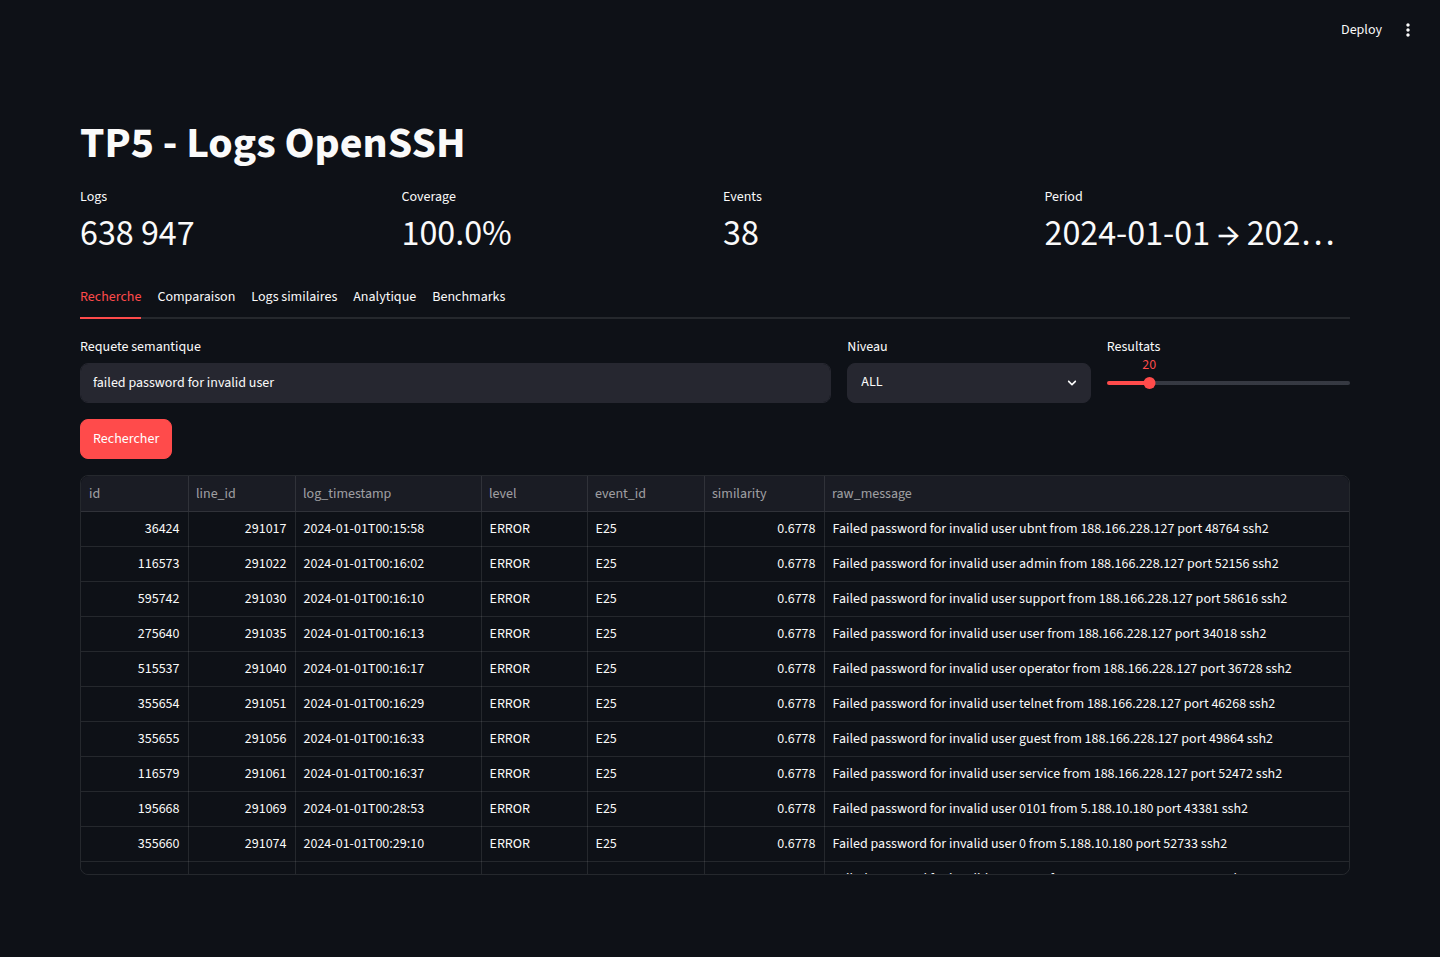
\includegraphics[width=\linewidth]{screenshots/02_semantic_search_results.png}
    \begin{center}\small Recherche semantique\end{center}
  \end{minipage}\hfill
  \begin{minipage}{0.48\linewidth}
    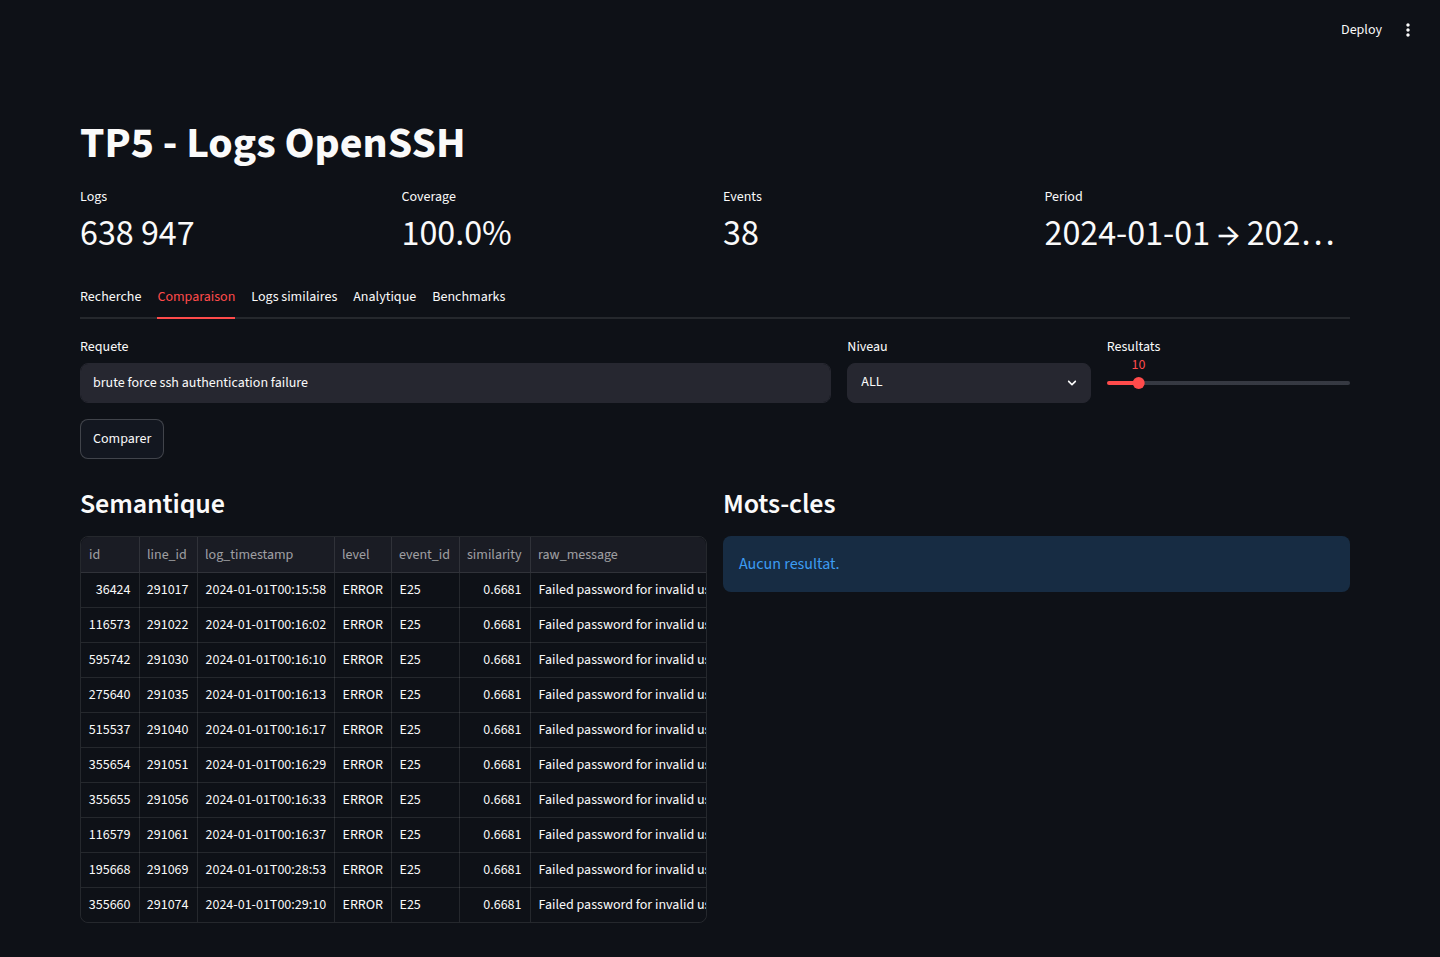
\includegraphics[width=\linewidth]{screenshots/03_semantic_keyword_comparison.png}
    \begin{center}\small Comparaison semantique/mots-cles\end{center}
  \end{minipage}

  \vspace{0.4cm}
  \begin{minipage}{0.48\linewidth}
    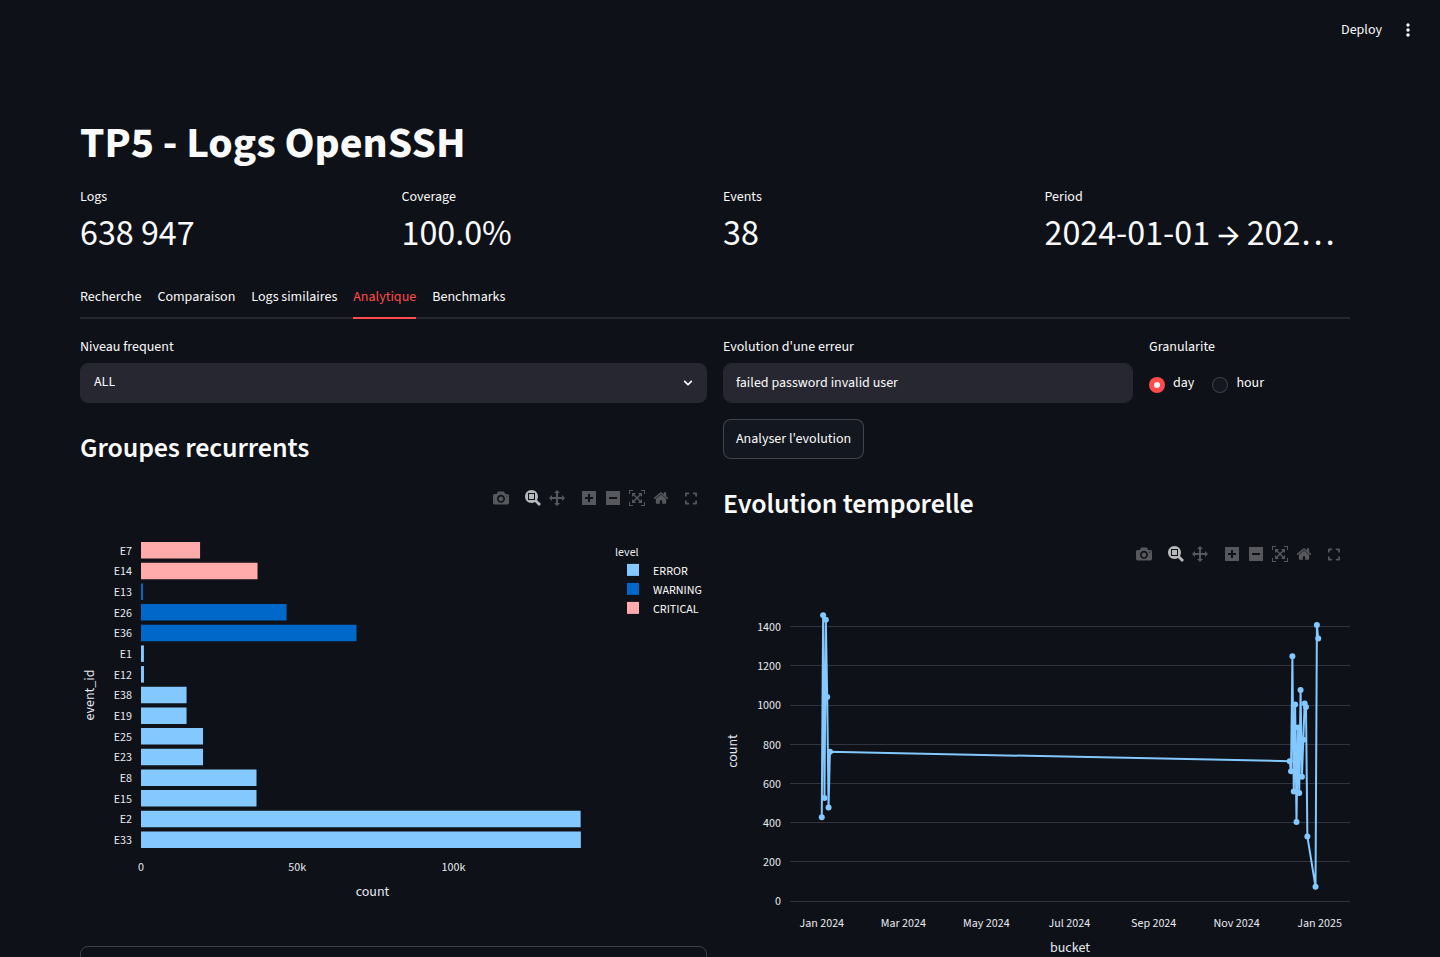
\includegraphics[width=\linewidth]{screenshots/05_analytics.png}
    \begin{center}\small Analytique des erreurs\end{center}
  \end{minipage}\hfill
  \begin{minipage}{0.48\linewidth}
    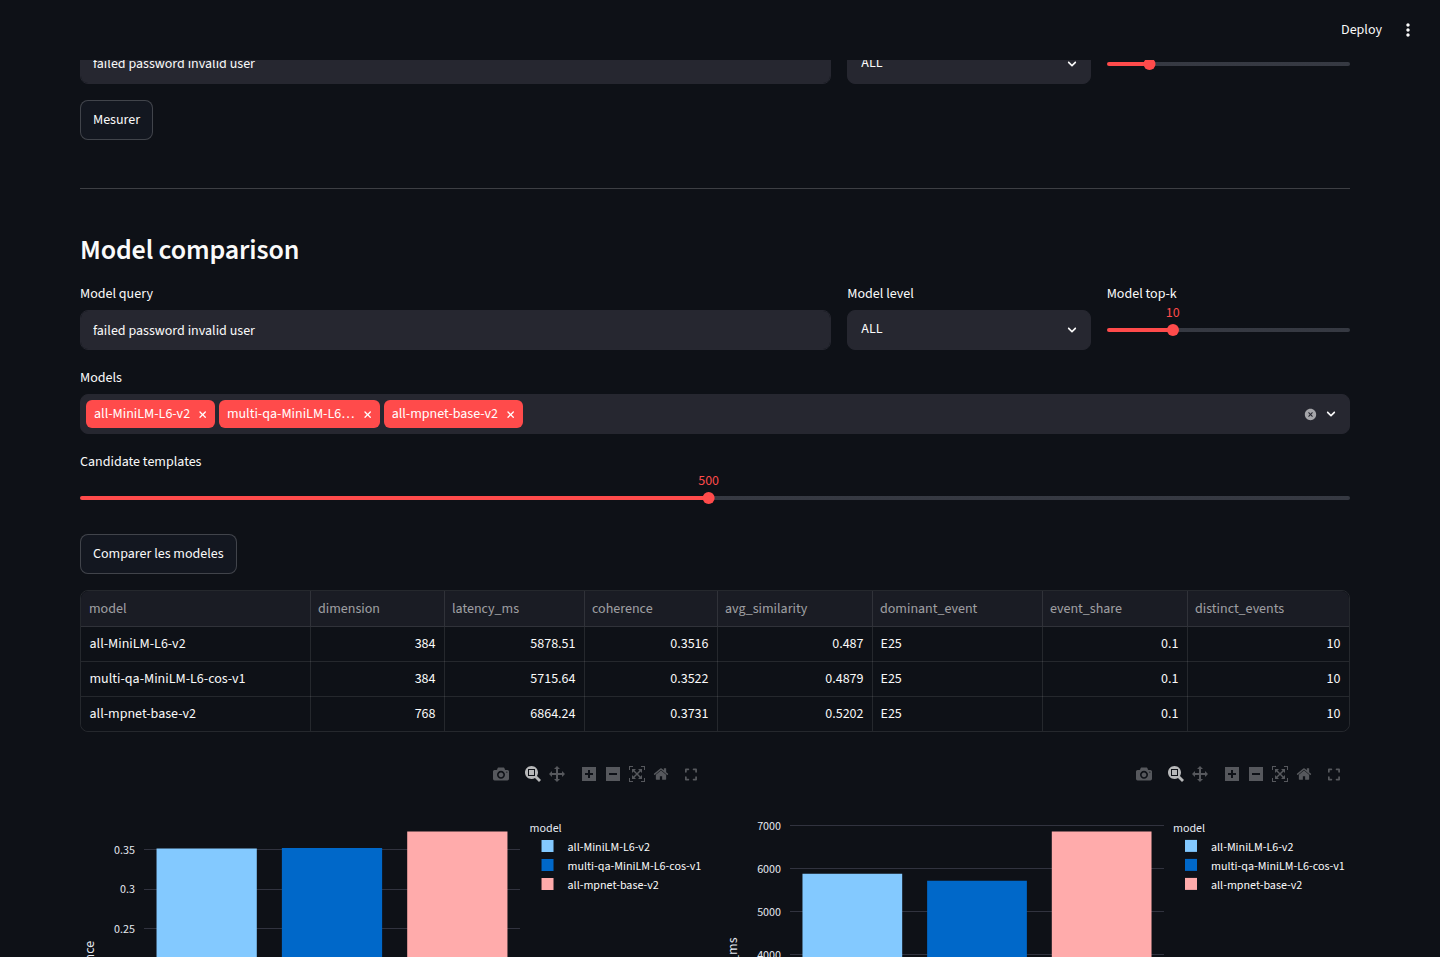
\includegraphics[width=\linewidth]{screenshots/07_model_comparison.png}
    \begin{center}\small Comparaison de modeles\end{center}
  \end{minipage}
\caption{Extraits de l'interface de visualisation.}
\end{figure}

\section{Validation des resultats}

La validation combine des criteres fonctionnels, techniques et qualitatifs. Sur le plan
fonctionnel, le systeme charge les donnees, remplit la base, vectorise les logs et retourne des
resultats exploitables depuis l'API et l'interface. Sur le plan technique, le pipeline reste
reproductible, le schema contient une colonne vectorielle indexee et les commandes principales sont
executables de maniere deterministe.

La qualite des resultats se verifie qualitativement. Pour une requete sur les echecs de mot de
passe, les premiers resultats appartiennent aux templates \texttt{Failed password} ou
\texttt{authentication failure}. Pour une requete sur les tentatives d'intrusion, les resultats font
apparaitre les messages de type \texttt{POSSIBLE BREAK-IN ATTEMPT} ou utilisateurs invalides. Pour
les analyses frequentes, les evenements les plus representes correspondent aux occurrences
indiquees par LogHub.

La performance depend de la machine. Le pretraitement Spark du dataset complet reste raisonnable sur
un poste local. La vectorisation par templates distincts reduit fortement le temps de calcul, car
elle evite de traiter plusieurs centaines de milliers de messages quasi identiques. La recherche
pgvector avec HNSW permet ensuite une latence compatible avec une interface interactive.
Les mesures ajoutees permettent de documenter cette performance avec des chiffres reproductibles
depuis l'API, la CLI ou l'interface web.

\section{Tests et validation}

Les tests unitaires valident le parsing OpenSSH, la normalisation des messages, la classification de
niveau, la conversion des vecteurs au format pgvector et le parsing de la CLI. Les tests
d'integration se font avec le pipeline limite, car ils impliquent Spark, PostgreSQL et le modele
d'embedding.

Les points verifies sont :

\begin{itemize}
  \item le pretraitement Spark produit les sorties CSV et Parquet ;
  \item PostgreSQL contient les logs et templates charges ;
  \item la table \texttt{message\_embeddings} couvre les messages normalises distincts ;
  \item l'index HNSW existe sur la table \texttt{message\_embeddings} ;
  \item une requete semantique retourne des messages OpenSSH coherents ;
  \item la comparaison mots-cles/semantique retourne deux listes distinctes ;
  \item l'onglet benchmarks affiche latence, tailles disque, coherence top-k et comparaison de modeles ;
  \item l'interface web communique avec l'API locale.
\end{itemize}

\section{Limites et ameliorations}

Le dataset OpenSSH ne contient pas l'annee dans le timestamp. L'annee configuree est donc une
hypothese technique pour permettre les analyses temporelles. Une extension possible serait de
croiser les logs avec une source externe contenant l'annee exacte.

La vectorisation par template est efficace et adaptee au dataset LogHub. Pour un environnement de
production avec des messages plus varies, on pourrait combiner deux niveaux de vecteurs : un vecteur
de template pour le regroupement et un vecteur de message brut pour la recherche fine.

Enfin, l'index HNSW privilegie la vitesse de recherche. Pour certaines evaluations, une recherche
exacte sans index pourrait servir de reference afin de mesurer le compromis entre performance et
rappel.

\section{Conclusion}

La plateforme constitue une chaine complete de recherche semantique et analytique sur logs massifs.
Spark
assure le traitement batch, PostgreSQL et pgvector fournissent la base vectorielle indexee,
Sentence-Transformers apporte la representation semantique, FastAPI expose les fonctionnalites et
Streamlit fournit l'interface de visualisation.

La solution couvre les cas d'utilisation principaux : retrouver les logs similaires a une erreur critique,
identifier les groupes d'erreurs frequentes, analyser leur evolution temporelle et comparer la
recherche semantique avec une recherche par mots-cles. Elle reste modulaire, reproductible et
adaptable a d'autres jeux de logs.

\end{document}
